\documentclass[9pt,handout]{beamer}
%\documentclass{beamer}

\usepackage{amsmath, epsfig, subfigure, psfrag, amssymb, amsfonts, array, amsthm}
\usepackage{tikz}
	\usetikzlibrary{calc, shapes.geometric, positioning, shapes, decorations, arrows, patterns}
\usepackage{wasysym}
 \usetikzlibrary{decorations.markings}

\mode<presentation>

\usetheme{Pittsburgh}
\usecolortheme{beaver}
%\useoutertheme{split}

\setbeamertemplate{footline}{}%[split, frame number]
\setbeamertemplate{enumerate items}[default]
\setbeamertemplate{itemize items}[circle]

\setbeamersize{text margin left=6mm}
\setbeamersize{text margin right=6mm}
\setbeamersize{sidebar width right=0mm}
\setbeamersize{sidebar width left=0mm}
\setbeamertemplate{navigation symbols}{}

\newtheorem{comments}{Comments}
\newtheorem{question}{Question}
\newtheorem{goal}{Goal}
\newtheorem{remark}{Remark}
\newtheorem{proposition}{Proposition}
\newtheorem{conjecture}{Conjecture}

% \newcommand*\oldmacro{}
% \let\oldmacro\insertshorttitle
% \renewcommand*\insertshorttitle{
% \oldmacro\hfill
% \insertframenumber\,/\,\inserttotalframenumber}

\def\tsimkappa{\sim_{\kappa}}
\def\r{\vec{r}}
\newcommand{\w}{\overline{w}}
%\DeclareMathOperator{\Cyc}{Acyc}
\DeclareMathOperator{\FC}{FC}
\newcommand{\C}{\widetilde{C}}
\DeclareMathOperator{\Sym}{Sym}
\DeclareMathOperator{\supp}{supp}
\newcommand{\LD}{\mathcal{L}}
\newcommand{\RD}{\mathcal{R}}

%%%%%%%%%%%%%% Heap Code %%%%%%%%%%%%%%
\usetikzlibrary{patterns}

\newcommand\heapblock[4]{\fill[fill=#4, fill opacity=0.35, draw=#4, line width=1.1pt, rounded corners,shift={(\xxaxis:#1)},shift={(\yyaxis:#2)}] (-1,-1) rectangle (1,1);\node at (#1,#2) {\footnotesize $#3$};}

\newcommand\dheapblock[4]{\draw[dotted, draw=#4, line width=1.1pt, rounded corners,shift={(\xxaxis:#1)},shift={(\yyaxis:#2)}] (-1,-1) rectangle (1,1);\node at (#1,#2) {\footnotesize $#3$};}

\newcommand\sheapblock[4]{\draw[pattern= north west lines, pattern color=#4, draw=#4, line width=1.1pt, rounded corners,shift={(\xxaxis:#1)},shift={(\yyaxis:#2)}] (-1,-1) rectangle (1,1);\node at (#1,#2) {\footnotesize $#3$};}

\newcommand\xxaxis{0}
\newcommand\yyaxis{90}

\definecolor{orange}{RGB}{255,102,0}
\definecolor{ggreen}{RGB}{0,153,0}
\definecolor{darkblue}{RGB}{0,0,255}
\definecolor{purple}{RGB}{153,51,255}
\definecolor{turq}{RGB}{72,209,204}
\definecolor{gray}{RGB}{220,220,220}
\definecolor{orange2}{RGB}{255,100,0}
\definecolor{purple2}{RGB}{159,51,250}
\definecolor{rred}{rgb}{0.9, 0.17, 0.31}


%% ----------------------------------------------------------------------  

\begin{document}

\def\newblock{\hskip .11em plus .33em minus .07em}

\title[A Study of T-Avoiding Elements in Coxeter Groups]
{\textbf{A Study of T-Avoiding Elements in Coxeter Groups}}
\author[T.M.~Laird]{Taryn Laird}
\institute[NAU]{Northern Arizona University\\
Department of Mathematics and Statistics}

\vspace{1em}

\date[NAU]{\textbf{NAU Thesis Defense}\\
April 29, 2016}

\frame{\titlepage}

%% ----------------------------------------------------------------------



\begin{frame}{\textbf{Coxeter Systems}}

\begin{definition}
A \alert{Coxeter system} consists of a group $W$ (called a \alert{Coxeter group}) generated by a set $S$ of involutions with presentation
\[ W=\langle S \mid s^2=e, (st)^{m(s,t)}=e \rangle \]

where $m(s,t) \geq 2$ for all $s \neq t$.
\end{definition}

\pause

\begin{block}{Comment}
Since $s$ and $t$ are involutions, the relation $(st)^{m(s,t)}=e$ can be 
rewritten as

\begin{center}
\begin{tabular}{ll}
$\left.\begin{array}{lcc}m(s,t)=2 & \implies &\ \ \, st=ts\ \   \end
{array}\right\}$&  \alert{commutations}\\
\\\pause
$\left.\begin{array}{lcc}m(s,t)=3 & \implies & sts=tst \\
& & \\
m(s,t)=4 & \implies & stst=tsts \\
 & \vdots &  \end{array}\right\}$ &\alert{braid relations}
\end{tabular}
\end{center}
\end{block}
\end{frame}

%% ----------------------------------------------------------------------

\begin{frame}{\textbf{Coxeter Graphs}}

\begin{definition}
We can encode $(W,S)$ with a unique \alert{Coxeter graph} $\Gamma$ having: 

\begin{itemize}
\item vertex set $S$;

\item edges $\{s,t\}$ labeled $m(s,t)$ whenever $m(s,t)\geq 3;$



\end{itemize}

\vspace{-1em}

\end{definition}

\pause

\begin{block}{Comments}
\begin{itemize}

\item if $m(s,t)=3$, we omit label.

\item If $s$ and $t$ are not connected in $\Gamma$, then $s$ and $t$ 
commute.

\item Given $\Gamma$, we can uniquely reconstruct the corresponding $(W,S)
$. 

\end{itemize}

\end{block}

\end{frame}

%% ----------------------------------------------------------------------

\begin{frame}{\textbf{Coxeter groups of type $A$}}

Coxeter groups of type $A_{n}$ ($n\geq 1$) are defined by:
\begin{figure}
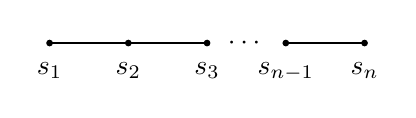
\begin{tikzpicture}
\draw[fill=black] \foreach \x in {1,2,3,4,5} {(\x,10) circle (1pt)};
\draw \foreach \x in {1,2,3} {(\x,10) node[label=below:$s_{\x}$]{}};
\draw {(4,10) node[label=below:$s_{n-1}$]{}};
\draw {(5,10) node[label=below:$s_{n}$]{}};
\draw {(3.5,10) node[]{$\cdots$}};
\draw[-] (1,10) -- (3,10);
\draw[-] (4,10) -- (5,10);
\end{tikzpicture}
\end{figure}

\pause
 
Then $W(A_{n})$ is generated by $\{s_{1}, s_{2}, \cdots, 
s_{n}\}$ and is subject to defining relations
\begin{enumerate}
\item $s_{i}^{2}=1$ for all $i$,
\item $s_{i}s_{j}=s_{j}s_{i}$ if $|i-j|>1$,
\item $s_{i}s_{j}s_{i}=s_{j}s_{i}s_{j}$ if $|i-j|=1$.
\end{enumerate}
\pause 
$W(A_{n})$ is isomorphic to the symmetric group, $Sym_{n+1}$, under 
the correspondence 
\[
s_{i}\mapsto (i,\ i+1),
\]
where $(i,\ i+1)$ is the adjacent transposition exchanging $i$ and $i+1$.

\end{frame}

%% ----------------------------------------------------------------------

\begin{frame}{\textbf{Coxeter groups of type $B$}}

Coxeter groups of type $B_{n}$ ($n\geq 2$) are defined by: 
\begin{figure}
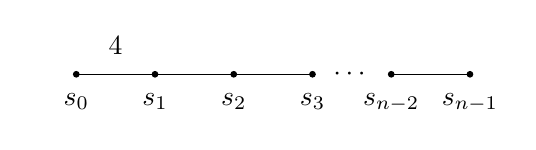
\begin{tikzpicture}[scale=1.0]%B_{n}
\draw [fill=black] \foreach \x in {1,2,...,6} {(\x,8.5) circle (1pt)};
%\draw [fill=white] (1,10) circle(2pt);
\draw {(.5,8.5) node{}
(1.5,8.5) node[label=above:$4$]{}
(6,8.5) node[label=above:\textcolor{white}{$4$}]{}
(4.5,8.5) node{$\cdots$}
(1,8.5) node[label=below:$s_0$]{}
(2,8.5) node[label=below:$s_1$]{}
(3,8.5) node[label=below:$s_2$]{}
(4,8.5) node[label=below:$s_3$]{}
(5,8.5) node[label=below:$s_{n-2}$]{}
(6,8.5) node[label=below:$s_{n-1}$]{}
[-] (1,8.5) -- (4,8.5)
[-] (5,8.5) -- (6,8.5)
(2,8.5) node{}}; 
\end{tikzpicture}
\end{figure}

\pause

Then $W(B_{n})$ is generated by $\{s_{1}, s_{2}, 
\cdots, s_{n-1}\}$ and is subject to defining relations 
\begin{enumerate}
\item $s_{i}^{2}=1$ for all $i$, 
\item $s_{i}s_{j}=s_{j}s_{i}$ if $|i-j|>1$, 
\item $s_{i}s_{j}s_{i}=s_{j}s_{i}s_{j}$ if $|i-j|=1$ and $1<i,j\leq n$, 
\item $s_{0}s_{1}s_{0}s_{1}=s_{1}s_{0}s_{1}s_{0}$.
\end{enumerate}
\pause $W(B_{n})$ is a finite group of order $n!2^{n}$ (wreath product of 
$\mathbb{Z}_{2}$ and the symmetric group).

\end{frame}

%% ----------------------------------------------------------------------


\begin{frame}{\textbf{Coxeter groups of type affine $C$}}

Coxeter groups of type $\C_{n}$ ($n \geq 2$) are defined by:
\begin{figure}
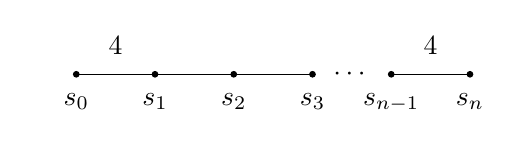
\begin{tikzpicture}[scale=1.0]
\draw[fill=black] \foreach \x in {1,2,...,6} {(\x,5) circle (1pt)};%\widetild{C}_{n}
%\fill[white] (1,6) circle (2pt);
\draw {(.5,5) node{}
(4.5,5) node{$\cdots$}
(5.5,5) node[label=above:$4$]{}
(1.5,5) node[label=above:$4$]{}
(1,5) node[label=below:$s_0$]{}
(2,5) node[label=below:$s_1$]{}
(3,5) node[label=below:$s_2$]{}
(4,5) node[label=below:$s_3$]{}
(5,5) node[label=below:$s_{n-1}$]{}
(6,5) node[label=below:$s_{n}$]{}
[-] (1,5) -- (4,5)
[-] (5,5) -- (6,5)
(2,5) node{}};
\end{tikzpicture}
\end{figure}

\pause 
Here, we see that $W(\C_{n})$ is generated by $\{s_{0}, 
\cdots, s_{n}\}$ and is subject to defining relations
\begin{enumerate}
\item $s_{i}^{2}=1$ for all $i$,
\item $s_{i}s_{j}=s_{j}s_{i}$ if $|i-j|>1$,
\item $s_{i}s_{j}s_{i}=s_{j}s_{i}s_{j}$ if $|i-j|=1$ and $1< i,j < n+1$, 
\item $s_{i}s_{j}s_{i}s_{j}=s_{j}s_{i}s_{j}s_{i}$ if $\{i,j\}=\{0,1\}$ or 
$\{n-1,n\}$.
\end{enumerate}
\pause 
\bigskip
$W(\C_{n})$ is an infinite group.

\pause

\begin{block}{Comment}
We can obtain $W(A_{n})$ and $W(B_{n})$ from $W(\C_{n})$ by removing the 
appropriate generators and corresponding relations.  In fact, 
we can obtain $W(B_{n})$ in two ways.
\end{block}

\end{frame}

%% ----------------------------------------------------------------------

\begin{frame}{\textbf{Reduced expressions}}

\begin{block}{Definition}
A word $s_{x_1}s_{x_2}\cdots s_{x_m}\in S^{*}$ is called an \alert
{expression} for $w\in W$ if it is equal to $w$ when considered as 
a group element.

\vspace{1em}
\pause

If $m$ is minimal, it is a \alert{reduced expression}, and the \alert
{length} of $w$ is $\ell(w):=m$.

\vspace{1em}
\pause

Given $w \in W$, if we wish to emphasize a fixed, possibly reduced, 
expression for $w$, we represent it as
\[
\w=s_{x_1}s_{x_2}\cdots s_{x_m}.
\]
\end{block}

\end{frame}

%% -------------------------------------------------------------------

\begin{frame}{\textbf{Matsumoto's Theorem and Support}}
\begin{block}{Theorem (Matsumoto)}
Any two reduced expressions for $w\in W$ differ by a sequence of commutations and braid moves.
\end{block}	

\pause

\begin{definition}
	We define $\supp(w)$ to be the set of generators appearing in any reduced expression for $w$. This is well defined by Matsumoto's theorem.
\end{definition}

\begin{definition}
 We define the \alert{left descent set} $w$ as follows:
\[\mathcal{L}(w):=\{s \in S \mid l(sw) < l(w)\}\]
\end{definition}


\pause

\begin{example}
Let $\w=s_2s_1s_2s_3s_1$ be a fixed expression for $w \in W(A_3)$. We see that
\[\alert{s_2s_1s_2}s_3s_1 \pause =s_1s_2s_1\alert{s_3s_1} \pause =s_1s_2\alert{s_1s_1}s_3\pause=s_1s_2s_3\]	
%This implies that $\w$ was not reduced. However, it turns out that $s_1s_2s_3$ is a reduced expression for $w$. Then $\supp(w)=\{s_1s_2s_3\}$ and $\ell(w)=3$.
\end{example}

\end{frame}


%% -------------------------------------------------------------------
\begin{frame}{\textbf{Fully Commutative Elements}}
\begin{definition}
Let $(W,S)$ be a Coxeter system of type $\Gamma$. We say that $w \in W(\Gamma)$ is \alert{fully commutative} (\alert{FC}) if any two reduced expressions for $w$ can be transformed into each other via iterated commutations. The set of FC elements is denoted $\FC(\Gamma)$.	
\end{definition}

\begin{block}{Theorem (Stembridge)}
$w \in \FC(\Gamma)$ if and only if no reduced expression for $w$ contains a braid.
\end{block}

\begin{block}{Comment}
	It follows from Stembridge that $W(\C_n)$ contains an infinite number of FC elements, while $W(A_n)$ and $W(B_n)$ do not. 
\end{block}

\end{frame}

%% -------------------------------------------------------------------

\begin{frame}{Fully Commutative Elements}
\begin{block}{Comment}
	The elements of $\FC(\C_n)$ are precisely those whose reduced expressions avoid the consecutive subwords $s_is_js_i$ for $m(s_i,s_j)=3$, $s_0s_1s_0s_1$, and $s_{n-1}s_ns_{n-1}s_n$.
\end{block}

\pause

\begin{block}{Example}
	Let $\w=s_0s_2s_4s_3s_2s_1$ be a reduced expression for $w \in W(\C_4)$. We see that
	\[s_0\alert{s_2s_4}s_3s_2s_1=s_0s_4\alert{s_2s_3s_2}s_1.\]
	Since $w$ has one of the forbidden consecutive subwords, $w$ is \alert{not} FC.
\end{block}
		
\end{frame}

%% -------------------------------------------------------------------

\begin{frame}{Heaps}
Every reduced expression $\w$ can be represented with a labeled partially ordered set (poset) called a heap, denoted $H(\w)$. Heaps provide a visual representation of a reduced expression while preserving the relations among the generators.

\pause

\begin{block}{Example}
Let $\w=s_4s_5s_1s_0s_2s_4s_1$ be a reduced expression for $w \in W(B_6)$.
\begin{columns}
\begin{column}{0.4\textwidth}
\begin{figure}\centering
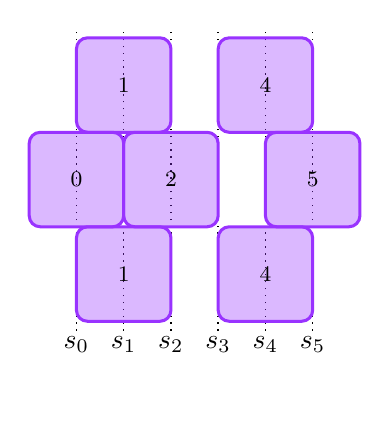
\begin{tikzpicture}[scale=0.6]
\node at (0.5,-2.5) {$ $};
\node at (0,-1.5) {$s_0$};
\node at (1,-1.5) {$s_1$};
\node at (2,-1.5) {$s_2$};
\node at (3,-1.5) {$s_3$};
\node at (4,-1.5) {$s_4$};
\node at (5,-1.5) {$s_5$};
\draw[dotted, line width=0.5pt] (1,-1.2) -- (1,5.2);
\draw[dotted, line width=0.5pt] (2,-1.2)   -- (2,5.2);
\draw[dotted, line width=0.5pt] (3,-1.2) -- (3,5.2);
\draw[dotted, line width=0.5pt] (4,-1.2)   -- (4,5.2);
\draw[dotted, line width=0.5pt] (5,-1.2) -- (5,5.2);
\draw[dotted, line width=0.5pt] (0,-1.2) -- (0, 5.2); 

\heapblock{1}{0}{1}{purple}
\heapblock{0}{2}{0}{purple}
\heapblock{2}{2}{2}{purple}
\heapblock{4}{0}{4}{purple}
\heapblock{1}{4}{1}{purple}
\heapblock{5}{2}{5}{purple}
\heapblock{4}{4}{4}{purple}

\end{tikzpicture}	
\end{figure}
\end{column}
\pause
\begin{column}{0.4\textwidth}
\begin{figure}\centering
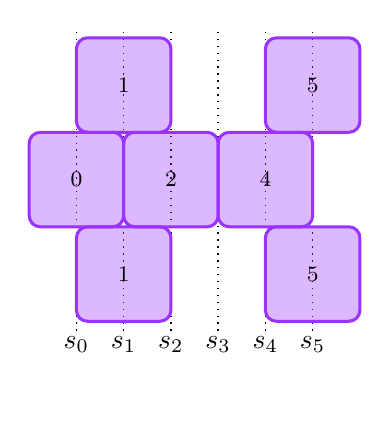
\begin{tikzpicture}[scale=0.6]
	\node at (0.5,-2.5) {$ $};
\node at (0,-1.5) {$s_0$};
\node at (1,-1.5) {$s_1$};
\node at (2,-1.5) {$s_2$};
\node at (3,-1.5) {$s_3$};
\node at (4,-1.5) {$s_4$};
\node at (5,-1.5) {$s_5$};
\draw[dotted, line width=0.5pt] (1,-1.2) -- (1,5.2);
\draw[dotted, line width=0.5pt] (2,-1.2)   -- (2,5.2);
\draw[dotted, line width=0.5pt] (3,-1.2) -- (3,5.2);
\draw[dotted, line width=0.5pt] (4,-1.2)   -- (4,5.2);
\draw[dotted, line width=0.5pt] (5,-1.2) -- (5,5.2);
\draw[dotted, line width=0.5pt] (0,-1.2) -- (0, 5.2); 

\heapblock{1}{0}{1}{purple}
\heapblock{0}{2}{0}{purple}
\heapblock{2}{2}{2}{purple}
\heapblock{5}{0}{5}{purple}
\heapblock{1}{4}{1}{purple}
\heapblock{4}{2}{4}{purple}
\heapblock{5}{4}{5}{purple}
\end{tikzpicture}
\end{figure}	
\end{column}
\end{columns}
\end{block}
	
\end{frame}

%% -------------------------------------------------------------------

\begin{frame}{Heaps}
\begin{block}{Theorem (Stembridge)}
	There is a unique heap for $w$ if and only if $w$ is FC.
\end{block}

\begin{block}{Lemma}
Let $w \in \FC(\C_n)$. Then $H(w)$ can not contain any of the following convex subheaps
\begin{columns}
	\begin{column}{0.1\textwidth}
	\begin{figure}{} \centering
	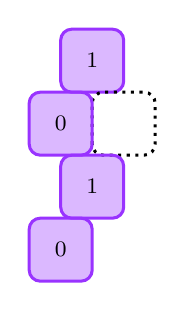
\begin{tikzpicture}[scale=0.4]
		\heapblock{1}{6}{1}{purple}
		\dheapblock{2}{4}{}{black}
		\heapblock{0}{4}{0}{purple}
		\heapblock{1}{2}{1}{purple}
		\heapblock{0}{0}{0}{purple}
	\end{tikzpicture}
	\end{figure} 
	\end{column}
	
	\begin{column}{0.1\textwidth}
	\begin{figure}{} \centering
	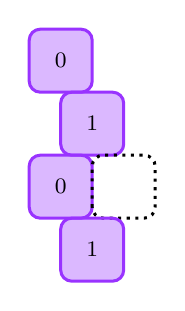
\begin{tikzpicture}[scale=0.4]
		\heapblock{0}{6}{0}{purple}
		\heapblock{1}{4}{1}{purple}
		\heapblock{0}{2}{0}{purple}
		\dheapblock{2}{2}{}{black}
		\heapblock{1}{0}{1}{purple}
	\end{tikzpicture}
	\end{figure} 
	\end{column}

\begin{column}{0.1\textwidth}
	\begin{figure} {} \centering
	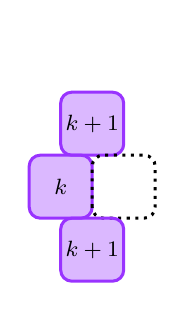
\begin{tikzpicture}[scale=0.4]
		\heapblock{1}{8}{}{white}
		\heapblock{1}{6}{k+1}{purple}
		\heapblock{0}{4}{k}{purple}
		\dheapblock{2}{4}{}{black}
		\heapblock{1}{2}{k+1}{purple}
	\end{tikzpicture}
	\end{figure}
	\end{column}
	
	\begin{column}{0.1\textwidth}
	\begin{figure}{} \centering
	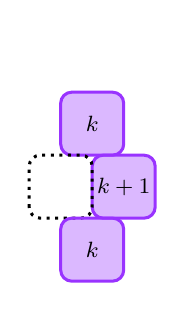
\begin{tikzpicture}[scale=0.4]
		\heapblock{1}{8}{}{white}
		\heapblock{2}{6}{k}{purple}
		\heapblock{3}{4}{k+1}{purple}
		\dheapblock{1}{4}{}{black}
		\heapblock{2}{2}{k}{purple}
	\end{tikzpicture}
	\end{figure}
	\end{column}
	
	\begin{column}{0.1\textwidth}
	\begin{figure}{} \centering
	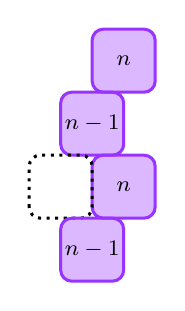
\begin{tikzpicture}[scale=0.4]
		\heapblock{2}{6}{n}{purple}
		\heapblock{1}{4}{n-1}{purple}
		\heapblock{2}{2}{n}{purple}
		\dheapblock{0}{2}{}{black}
		\heapblock{1}{0}{n-1}{purple}
	\end{tikzpicture}
	\end{figure}
	\end{column} 
	
	\begin{column}{0.1\textwidth}
	\begin{figure}{} \centering
	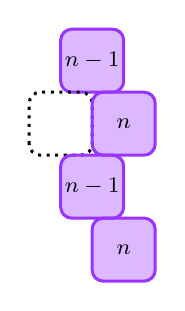
\begin{tikzpicture}[scale=0.4]
		\heapblock{1}{6}{n-1}{purple}
		\dheapblock{0}{4}{}{black}
		\heapblock{2}{4}{n}{purple}
		\heapblock{1}{2}{n-1}{purple}
		\heapblock{2}{0}{n}{purple}
	\end{tikzpicture}	
	\end{figure}
	\end{column}	
\end{columns}
\end{block}
	
\end{frame}

%% -------------------------------------------------------------------

\begin{frame}{Star Reductions}
\begin{block}{Definition}
	We define $w$ to be \alert{left star reducible by $s$ with respect to $t$} if $m(s,t) \geq 3$, $s \in \LD(w)$ and $ t \in \LD(sw)$.
\end{block}

\pause

\begin{columns}
\begin{column}{0.4\textwidth}
\begin{figure} \centering
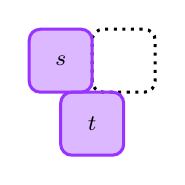
\begin{tikzpicture}[scale=0.4]
	\dheapblock{2}{2}{}{black}
	\heapblock{0}{2}{s}{purple}
	\heapblock{1}{0}{t}{purple}
\end{tikzpicture}
\end{figure}	
\end{column}
	
\begin{column}{0.4\textwidth}	
\begin{figure}
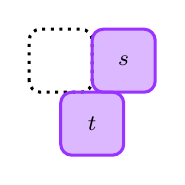
\begin{tikzpicture}[scale=0.4]
	\dheapblock{1}{2}{}{black}
	\heapblock{3}{2}{s}{purple}
	\heapblock{2}{0}{t}{purple}
\end{tikzpicture}	
\end{figure}
\end{column}
\end{columns}

\pause

\begin{block}{Definition}
	We define $W(\Gamma)$ to be \alert{star reducible} if every element of $\FC(\Gamma)$ is star reducible to a product of commuting generators.
\end{block}

\pause

\begin{block}{Theorem (Green)}
	Coxeter systems of type $A_n$ $(n \geq 1)$, type $B_n$ $(n \geq 2)$, type $D_n$ $(n \geq 4)$, type $F_n$ $(n \geq 4)$, type $H_n$ $(n \geq 2)$, type $I_2(m)$ $(m \geq 3)$, type $\widetilde{A}_{n}$ $(n \geq 3 \text{ and } n \text{ even })$, type $\widetilde{C}_{n}$ $(n\geq 3 \text{ and } n \text{ odd })$, type $\widetilde{E}_6$, or type $\widetilde{F}_5$, are star reducible.
\end{block}
	
\end{frame}


%% -------------------------------------------------------------------

\begin{frame}{Property T}
	\begin{block}{Definition}
	We define $w$ to have \alert{Property T} if and only if there exists a reduced product for $w$ such that $w=stu$ or $w=uts$ where $m(s,t) \geq 3$. \pause 
	
	We say $w$ is \alert{T-avoiding} if $w$ does not have Property T.
	\end{block}

\begin{block}{Proposition}
A product of commuting generators is T-avoiding.	
\end{block}

\begin{block}{Definition}
	We define $w$ to be \alert{trivially T-avoiding} if $w$ is a product of commuting generators. Otherwise, we say $w$ is \alert{non-trivially T-avoiding}.
\end{block}

\end{frame}


%% -------------------------------------------------------------------


\begin{frame}{Examples of Property T and T-avoiding}

\begin{block}{Example}
Let $\w_1=s_5s_3s_2s_4s_1$ be a reduced expression for $w \in W(A_5)$. 
\pause
\begin{figure}
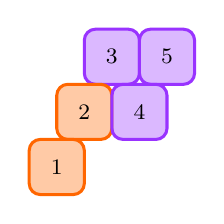
\begin{tikzpicture}[scale=0.35]
\heapblock{5}{6}{5}{purple}
\heapblock{3}{6}{3}{purple}
\heapblock{2}{4}{2}{orange}
\heapblock{4}{4}{4}{purple}
\heapblock{1}{2}{1}{orange}
\end{tikzpicture}	
\end{figure}
\end{block}

\pause

\begin{block}{Example}
Let $\w_2=s_0s_2s_4s_1s_3s_0s_2s_4$ be a reduced expression for $w \in W(\C_4)$.
\begin{figure}
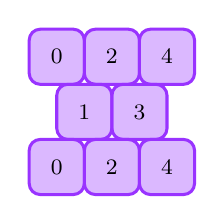
\begin{tikzpicture}[scale=0.35]
\heapblock{0}{6}{0}{purple}
\heapblock{2}{6}{2}{purple}
\heapblock{4}{6}{4}{purple}
\heapblock{1}{4}{1}{purple}
\heapblock{3}{4}{3}{purple}
\heapblock{0}{2}{0}{purple}
\heapblock{2}{2}{2}{purple}
\heapblock{4}{2}{4}{purple}
\end{tikzpicture}	
\end{figure}
\end{block}

\end{frame}


%% -------------------------------------------------------------------


\begin{frame}{Classification of T-Avoiding Elements: Already Known $\widetilde{A}_n$}

\begin{block}{Theorem (Fan)}
	If $n$ is odd, and $n \geq 2$ there are no non-trivial T-avoiding elements in $W(\widetilde{A}_n)$. If $n$ is even, and $n \geq 2$ then $W(\widetilde{A}_n)$ contains non-trivial T-avoiding elements.
\end{block}
\pause
\begin{block}{Conjecture}
The only non-trivial T-avoiding elements of $W(\widetilde{A}_n)$ for $n$ odd are of the form $w=(s_0s_2 \cdots s_{n-2}s_ns_1s_3 \cdots s_{n-3}s_{n-1})^k$  for $k \in \mathbb{Z}^+$.	
\end{block}
\pause
\begin{block}{Theorem}
There are no non-trivial T-avoiding elements in $W(A_n)$.	
\end{block}

\end{frame}


%% -------------------------------------------------------------------


\begin{frame}{Classification of T-Avoiding Elements : Already Known $D_n$}

\begin{block}{Theorem (Gern)}
There are non-trivial T-avoiding elements in $W(D_n)$.	
\end{block}
\pause
\begin{figure}
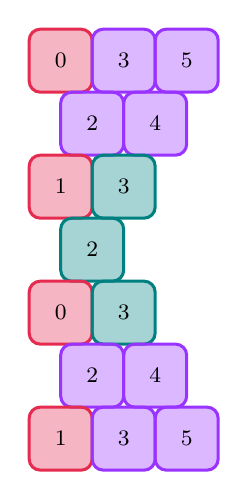
\begin{tikzpicture}[scale=0.4]
	\heapblock{1}{12}{0}{rred}
	\heapblock{3}{12}{3}{purple}
	\heapblock{5}{12}{5}{purple}
	\heapblock{2}{10}{2}{purple}
	\heapblock{4}{10}{4}{purple}
	\heapblock{1}{8}{1}{rred}
	\heapblock{3}{8}{3}{teal}
	\heapblock{2}{6}{2}{teal}
	\heapblock{1}{4}{0}{rred}
	\heapblock{3}{4}{3}{teal}
	\heapblock{2}{2}{2}{purple}
	\heapblock{4}{2}{4}{purple}
	\heapblock{1}{0}{1}{rred}
	\heapblock{3}{0}{3}{purple}
	\heapblock{5}{0}{5}{purple}
\end{tikzpicture}
\end{figure}
	
\end{frame}


%% -------------------------------------------------------------------


\begin{frame}{Classification of T-Avoiding Elements: Already Known $F_n$}

\begin{block}{Theorem (Cross, Ernst, Hills-Kimball, Quaranta)}
The only non-trivial T-avoiding elements in $F_5$ are stacks of bowties.	
\end{block}

\begin{figure}
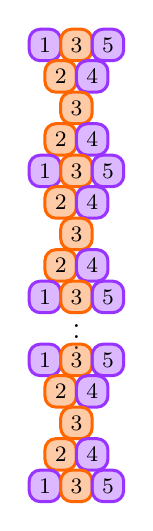
\begin{tikzpicture}[scale=0.2]
\heapblock{1}{10}{1}{purple}
	\heapblock{3}{10}{3}{orange}
	\heapblock{5}{10}{5}{purple}
	\heapblock{2}{8}{2}{orange}
	\heapblock{4}{8}{4}{purple}
	\heapblock{3}{6}{3}{orange}
	\heapblock{2}{4}{2}{orange}
	\heapblock{4}{4}{4}{purple}
	\heapblock{1}{2}{1}{purple}
	\heapblock{3}{2}{3}{orange}
	\heapblock{5}{2}{5}{purple}
	\heapblock{2}{0}{2}{orange}
	\heapblock{4}{0}{4}{purple}
	\heapblock{3}{-2}{3}{orange}
	\heapblock{2}{-4}{2}{orange}
	\heapblock{4}{-4}{4}{purple}
	\heapblock{1}{-6}{1}{purple}
	\heapblock{3}{-6}{3}{orange}
	\heapblock{5}{-6}{5}{purple}
	
	\node[] at (3,-8){$\vdots$};
	
	\heapblock{1}{-10}{1}{purple}
	\heapblock{3}{-10}{3}{orange}
	\heapblock{5}{-10}{5}{purple}
	\heapblock{2}{-12}{2}{orange}
	\heapblock{4}{-12}{4}{purple}
	\heapblock{3}{-14}{3}{orange}
	\heapblock{2}{-16}{2}{orange}
	\heapblock{4}{-16}{4}{purple}
	\heapblock{1}{-18}{1}{purple}
	\heapblock{3}{-18}{3}{orange}
	\heapblock{5}{-18}{5}{purple}
\end{tikzpicture}
\end{figure}
 	
\end{frame}


%% -------------------------------------------------------------------

\begin{frame}{Classification of T-Avoiding Elements: Already Known $F_n$}

\begin{block}{Corollary (Cross, Ernst, Hills-Kimball, Quaranta)}
There are no non-trivial T-avoiding elements in $F_4$.	
\end{block}
\pause
Classifying non-trivial T-avoiding elements in $F_n$ for $n \geq 6$ gets very difficult.
\pause
\begin{figure}\centering
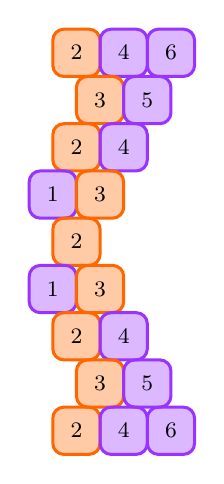
\begin{tikzpicture}[scale=0.3]
	\heapblock{2}{10}{2}{orange}
	\heapblock{4}{10}{4}{purple}
	\heapblock{6}{10}{6}{purple}
	\heapblock{3}{8}{3}{orange}
	\heapblock{5}{8}{5}{purple}
	\heapblock{2}{6}{2}{orange}
	\heapblock{4}{6}{4}{purple}
	\heapblock{1}{4}{1}{purple}
	\heapblock{3}{4}{3}{orange}
	\heapblock{2}{2}{2}{orange}
	\heapblock{1}{0}{1}{purple}
	\heapblock{3}{0}{3}{orange}
	\heapblock{2}{-2}{2}{orange}
	\heapblock{4}{-2}{4}{purple}
	\heapblock{3}{-4}{3}{orange}
	\heapblock{5}{-4}{5}{purple}
	\heapblock{2}{-6}{2}{orange}
	\heapblock{4}{-6}{4}{purple}
	\heapblock{6}{-6}{6}{purple}
\end{tikzpicture}
\end{figure}

\end{frame}


%% -------------------------------------------------------------------


\begin{frame}{Classification of T-Avoiding Elements: $I_2(m)$}

\begin{block}{Theorem}
	There are no non-trivial T-avoiding elements in $W(I_2(m))$.
\end{block}

\end{frame}


%% -------------------------------------------------------------------


\begin{frame}{Signed Permutation Representation}

Since $W(B_n) \cong \Sym_n^B$, we can write $w \in W(B_n)$ as a signed permutation 
\[[w(1), w(2), \ldots, w(n)]\] where we write a bar underneath a number in place of a negative sign.

\pause

\begin{block}{Definition}
	We 
\end{block}

	
\end{frame}


%% -------------------------------------------------------------------


\begin{frame}{Classification of T-Avoiding Elements: $B_n$}

\begin{block}{Theorem (Laird)}
	There are no non-trivial T-avoiding elements in $W(B_n)$.
\end{block}

\end{frame}




\end{document}